\documentclass[10pt]{scrartcl}
\usepackage{graphicx}
\usepackage[default]{opensans}
\usepackage{sfmath} % sans font also for math
 \usepackage[binary-units = true]{siunitx}

% defining the paper layout that no text overlaps with the header
\usepackage[
  top=35mm,
  headheight=25mm,
  headsep=3mm,
  bottom=30mm,
  left=25mm,
  right=25mm
]{geometry}

\usepackage{latexsym}
\usepackage[centertags]{amsmath}
\usepackage{amssymb}

% custom header and footpage
\usepackage{scrpage2}
\pagestyle{scrheadings} % you have to set the custom layout
\ihead{} % left head
\ohead{
\includegraphics[height=25mm]{EUCALL.png}}
\ifoot{
\includegraphics[height=13.4mm]{EU.png}} % left foot
\cfoot{
  \begin{minipage}{100mm}
    \begin{scriptsize}
      \normalfont{This project has received funding from the}
      \textit{European Union’s Horizon 2020 research and innovation programme}
      \normalfont{under grant agreement No 654220.}
    \end{scriptsize}
  \end{minipage}
} % center foot
\ofoot{\thepage} % right foot
\chead{}

\usepackage{booktabs} % more eye candy for tables

% sophisticated linking of references in the pdf and setting some options
\usepackage{url}                                                  % for correct typesettings of URLs
\usepackage{hyperref}                                             % for sophisticated linking of urls, dois, pictures, tables, etc.
\hypersetup{
    unicode=true,                                                 % non-Latin characters in Acrobat’s bookmarks
    pdftoolbar=true,                                              % show Acrobat’s toolbar?
    pdfmenubar=true,                                              % show Acrobat’s menu?
    pdffitwindow=false,                                           % window fit to page when opened
    pdfstartview={FitH},                                          % fits the width of the page to the window
    pdftitle={D4.4: Interoperable simulations},                                        % title
    pdfauthor={C. Fortmann-Grote},                                           % author
    pdfsubject={EUCALL WP4 (SIMEX) Deliverable D4.4},                             % subject of the document
    pdfcreator={pdflatex},                                         % creator of the document
    pdfkeywords={EUCALL, SIMEX, simulations, Rad-Hydro, XFEL, ESRF, warm dense
    matter, absorption, radiography},                                         % list of keywords
    pdfnewwindow=true,                                            % links in new PDF window
    colorlinks=true,                                              % false: boxed links; true: colored links
    linkcolor=blue,                                                % color of internal links (change box color with linkbordercolor)
    citecolor=blue,                                                % color of links to bibliography
    filecolor=blue,                                               % color of file links
    urlcolor=blue                                                 % color of external links
}

% Zeilenabstand
\renewcommand{\baselinestretch}{1.2}


%\renewcommand*\chapterpagestyle{scrheadings} % otherwise chapter start is plain ;-); works only for KOMA script; plain LaTeX works different

%%%%%%%%%%%%%%%%%%%%%%%%%%%%%%%%%%%%%%%%%%%%%%%
%   BIBLIOGRAPHY SETTINGS                     %
%%%%%%%%%%%%%%%%%%%%%%%%%%%%%%%%%%%%%%%%%%%%%%%
\usepackage[bibstyle=nature,sorting=none,maxnames=1000,eprint=false,
defernumbers=true, backend=biber]{biblatex}
\usepackage{hyperref}

\renewcommand*\finalnamedelim{, and\addspace}
\DeclareNameAlias{sortname}{last-first}
\renewcommand{\newunitpunct}{, }

\AtEveryBibitem{%
  \clearfield{day}%
  \clearfield{month}%
  \clearfield{endday}%
  \clearfield{endmonth}%
  \clearfield{issn}%
  \clearfield{issue}%
}
%convert titles to hyperlinks using doi
\ExecuteBibliographyOptions{doi=false} \newbibmacro{string+doi}[1]{%
  \iffieldundef{doi}{#1}{\href{http://dx.doi.org/\thefield{doi}}{#1}}}
  \DeclareFieldFormat*{title}{\usebibmacro{string+doi}{\mkbibemph{#1}}}

\addbibresource{references.bib}
\addbibresource{urls.bib}
\addbibresource{aux.bib}
%%%%%%%%%%%%%%%%%%%%%%%%%%%%%%%%%%%%%%%%%%%%%%%
% END BIBLIOGRAPHY SETTINGS                   %
%%%%%%%%%%%%%%%%%%%%%%%%%%%%%%%%%%%%%%%%%%%%%%%

\begin{document}
\makeatletter
\begin{titlepage}
\thispagestyle{scrheadings}
\begin{center}
$~$\\
\vspace{0cm}
{\Large\textbf{EUCALL}\\[2ex]
The European Cluster of Advanced Laser Light Sources}\\[4ex]
%
{\small\textbf{Grant Agreement number: 654220}}\\[8ex]
%
Work Package 4 -- SIMEX\\[4ex]
%
Deliverable D4.4\\
%
Simulated coherent scattering data from plasma and non--plasma samples\\[5ex]
%
Lead Beneficiary: European XFEL, HZDR\\[5ex]
%
Carsten Fortmann-Grote, Michael Bussmann,
  Marco Garten, Axel Huebl, Thomas Kluge,
  and Adrian P. Mancuso\\[4ex]
%
Due data: September 30, 2017\\
Date of delivery: \today \\[4ex]
%
Project webpage: \url{www.eucall.eu}\\[6ex]
%
{%
\small
\begin{tabular}{|l|l|}
  \hline
  \multicolumn{2}{|l|}{ \textit{Deliverable Type} } \\
  \hline
  R = Report\hfill & R, OTHER \\
  DEM = Demonstrator, pilot, prototype, plan designs & \\
  DEC = Websites, patents filing, press \& media actions, videos, etc. & \\
  OTHER = Software, technical diagram, etc. & \\
  \hline
  \multicolumn{2}{|l|}{\textit{Dissemination level}} \\
  \hline
  PU = Public, fully open, e.g. web & PU \\
  CO = Confidential, restricted under conditions set out in Model Grant
  Agreement\hspace*{17ex}\  & \\
  CI = Classified, information as referred to in Commission Decision 2001/844/EC
  & \\
  \hline
\end{tabular}
}

\end{center}
%
%\vfill
\centering{%
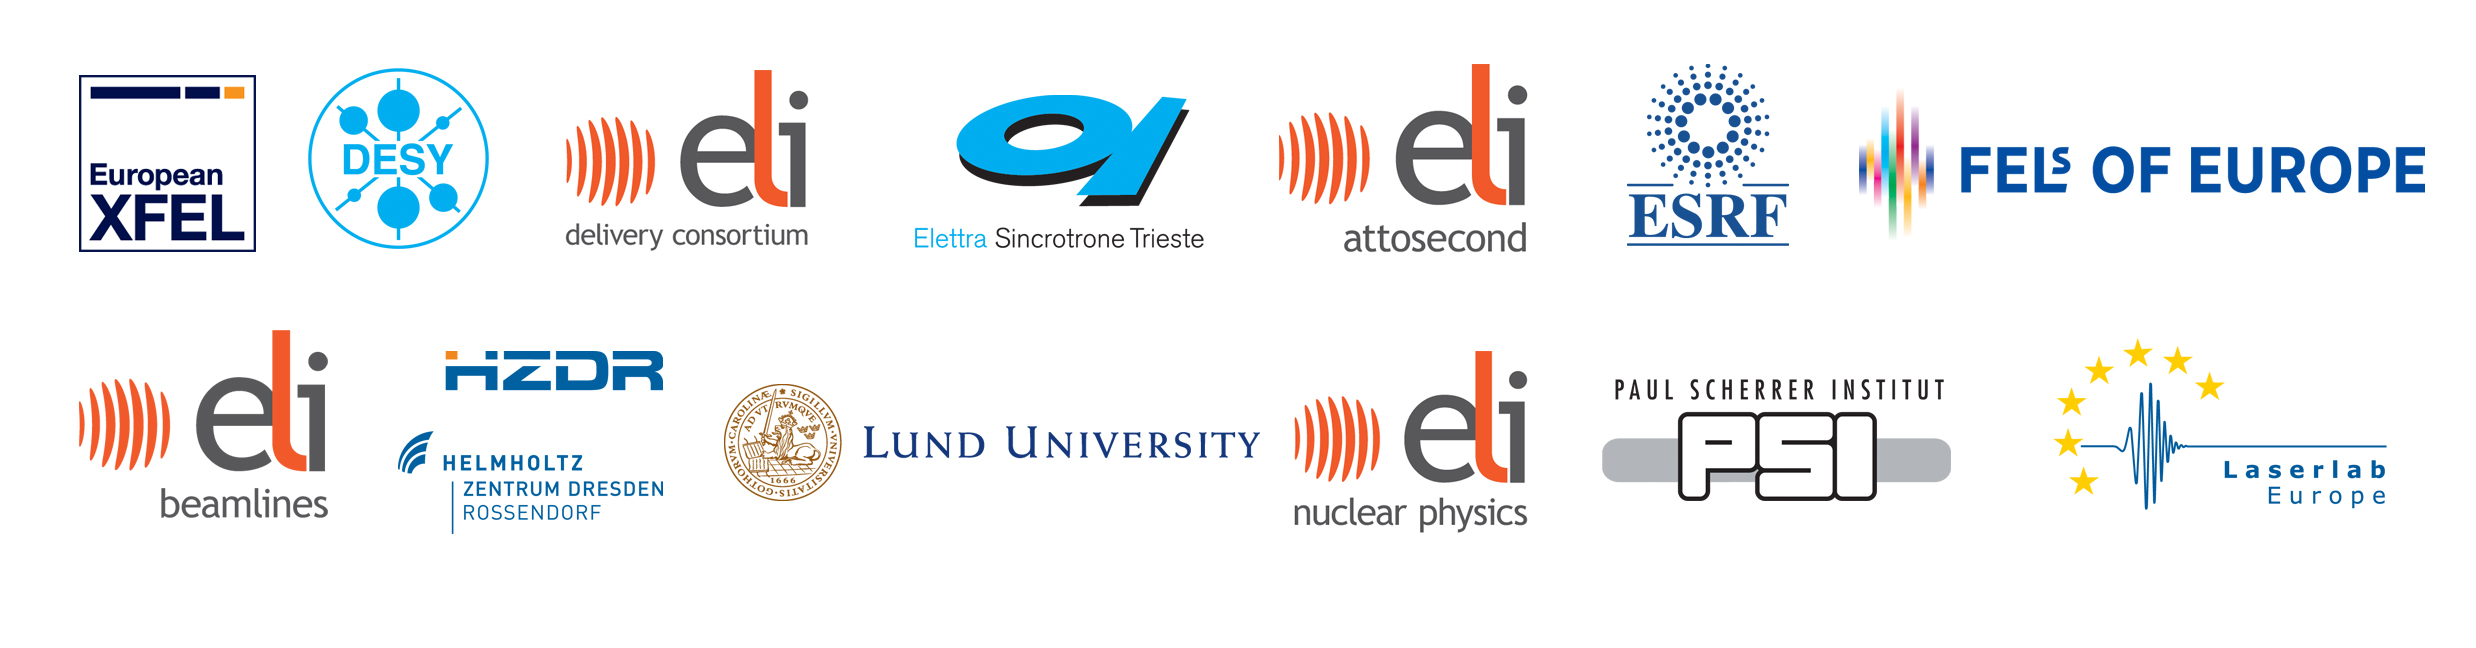
\includegraphics[width=0.91\textwidth]{figures/PartnerLogos_2017}
}
\normalfont
\end{titlepage}
\makeatother

%\tableofcontents

\section{Summary}
%
As first applications, we have employed the simulation capabilities of
\textit{simex\_platform} \cite{simex_github} to simulate two photon experiments:
\begin{enumerate}
  \item Coherent diffraction from high--power laser excited optically thin and
    thick plasmas (plasma sample)
  \item Single particle imaging at the European XFEL (non--plasma sample)
\end{enumerate}

\section{Plasma sample}
The virtual experiment is described in detail in section 4 of the EUCALL
Milestone M4.3~\cite{EUCALL_SIMEX_M4.3}. The resulting datasets for scattering
from optically thin and thick plasmas are published on the
\href{https://www.zenodo.org/communities/eucall-data}{EUCALL Data Repository}
\cite{Garten2017.zenodo.885033}.

\section{Molecular (non--plasma) sample}
Application of \textit{simex\_platform} to single--particle imaging experiments
at the European X--ray Free Electron Laser (SPB--SFX scientific instrument) has
been published as Ref.~\cite{Fortmann-Grote2017}. It is also the basis for an
online tutorial on the
\href{https://www.github.com/eucall-software/simex_platform/wiki/SimEx-Tutorial}{wiki
pages} of \textit{simex\_platform} and it is
discussed in the EUCALL Milestone M4.2~\cite{EUCALL_SIMEX_M4.2} (First example
simulation).
The datasets for coherent diffraction from the protein 2NIP is deposited on
the \href{https://www.zenodo.org/communities/eucall-data}{EUCALL Data
Repository} \cite{Fortmann-Grote2017.zenodo.886087}.


\printbibliography
%%%%%%%%%%%%%%%%%%%%%%%%%%%
\end{document}


